To solve the constrained optimization problem \eqref{eq:disoTPS_YB_move_alternative_formulation} we proceed by maximizing the overlap while only varying the parameters of one of the three tensors $T^\prime$, $W_1^\prime$ or $W_2^\prime$, keeping all other tensors fixed. We can then iterate over the three tensors to converge to a solution. \par
Tensor diagrams for the algorithm are shown in figure \figref{fig:YB_move_iterate_polar}. We first show how the tensor $W_2^\prime$ can be optimized. We treat all tensors except $W_2^\prime$ as constant and contract them into an environment $E$ as shown in figure \figref{fig:YB_move_iterate_polar_optimize_W2}. One can then write the optimization problem as
\begin{equation}
	\label{eq:disoTPS_YB_move_optimization_problem_W_2_prime}
	W_2^\prime = \underset{\lVert W_1^\prime \rVert = 1}{\text{argmax}} \Re\left\langle\Psi\middle|\Psi^\prime\right\rangle = \underset{\lVert W_1^\prime \rVert = 1}{\text{argmax}} \Re\left\langle W_2^\prime, E \right\rangle_\text{F},
\end{equation}
with the Frobenius inner product $\left\langle \cdot, \cdot \right\rangle_\text{F}$ \eqref{eq:frobenius_inner_product}. The Frobenius inner product satisfies the Cauchy-Schwarz inequality and we obtain
\begin{equation}
	\left|\Re\left\langle W_2^\prime, E \right\rangle_\text{F}\right| \le \lVert W_2^\prime\rVert\lVert E\rVert = \lVert E\rVert.
\end{equation}
If we set $W = E/\lVert E\rVert$ we obtain
\begin{equation}
	\Re\left\langle W_2^\prime, E \right\rangle_\text{F} = \frac{\Re\left\langle E^\prime, E \right\rangle_\text{F}}{\lVert E\rVert} = \lVert E\rVert
\end{equation}
and the maximum is reached. Thus, the closed form solution to \eqref{eq:disoTPS_YB_move_optimization_problem_W_2_prime} is $W_2^\prime = E/\lVert E\rVert$. \par
Next, we optimize the tensor $W_1^\prime$. Again, we keep all other tensors fixed and contract them into the environment $E$ as shown in figure \figref{fig:YB_move_iterate_polar_optimize_W1}. We now reshape $E$ into a matrix, grouping together all legs that connect to legs of $W_1^\prime$ decorated with incoming/outgoing arrows respectively (see figure \figref{fig:YB_move_iterate_polar_optimize_W1}). For the bond dimensions specified in figure \figref{fig:YB_move_iterate_polar_overlap}, $E$ is a complex $\chi D^2 \times \chi$ matrix. The optimization problem can then be written as
\begin{equation}
	\label{eq:disoTPS_YB_move_optimization_problem_W_1_prime}
	W_1^\prime = \underset{W_1^{\prime\dagger}W_1^\prime = \id}{\text{argmax}}\Re\left\langle\Psi\middle|\Psi^\prime\right\rangle = \underset{W_1^{\prime\dagger}W_1^\prime = \id}{\text{argmax}} \Re\left\langle W_1^\prime, E \right\rangle_\text{F} = \underset{W_1^{\prime\dagger}W_1^\prime = \id}{\text{argmax}} \Re\Tr\left(W_1^{\prime\dagger}E\right),
\end{equation}
where $W_1^\prime$ has the same dimensions as $E$. This is known as the \textit{orthogonal procrustes problem} and permits a closed-form solution. \todo{cite something for the procrustes problem?} Taking the SVD of $E$ yields $E = USV^\dagger$. Note that, because of the shape of $E$, $V$ is a unitary matrix of shape $\chi\times\chi$. Inserting the SVD into the trace yields
\begin{equation}
	\begin{split}
		\Re\Tr\left(W_1^{\prime\dagger}E\right) &= \Re\Tr\left(E W_1^{\prime\dagger}\right) = \Re\Tr\left(USV^\dagger W_1^{\prime\dagger}\right)\\
		&= \Re\Tr\left[\left(U\sqrt{S}\right)\left(\sqrt{S}V^\dagger W_1^{\prime\dagger}\right)\right] = \Re\left\langle\sqrt{S}U^\dagger,\sqrt{S}V^\dagger T^{\prime\dagger}\right\rangle_\text{F}.
	\end{split}
\end{equation}
We again use the Cauchy-Schwarz inequality to obtain an upper bound
\begin{equation}
	\begin{split}
		\left|\Re\Tr\left(W_1^{\prime\dagger}E\right)\right| &= \left|\Re\left\langle\sqrt{S}U^\dagger,\sqrt{S}V^\dagger T^{\prime\dagger}\right\rangle_\text{F}\right| \le \left\lVert\sqrt{S}U^\dagger\right\rVert_\text{F} \left\lVert\sqrt{S}V^\dagger T^{\prime\dagger}\right\rVert_\text{F}\\
		&= \sqrt{\Tr\left(USU^\dagger\right)\Tr\left(T^\prime VSV^\dagger T^{\prime\dagger}\right)} = \Tr\left(S\right),		
	\end{split}
\end{equation}
where in the last step we used $U^\dagger U = \id$, $V^\dagger V = \id$, $W_1^{\prime\dagger}W_1^\prime = \id$ and the cyclic property of the trace. The upper bound can be reached by setting $W_1^\prime = UV^\dagger$:
\begin{equation}
	\Re\Tr\left(W_1^{\prime\dagger}E\right) = \Re\Tr\left(VU^\dagger USV^\dagger\right) = \Tr\left(S\right).
\end{equation}
Thus, the closed form solution to \eqref{eq:disoTPS_YB_move_optimization_problem_W_1_prime} is $W_1^\prime = UV^\dagger$. \par
Lastly we show how the tensor $T^\prime$ can be optimized. Similar to the optimization of $W_1^\prime$, we obtain an orthogonal Procrustes problem after contracting the environment $E$ and performing an SVD $E = USV^\dagger$ as shown in figure \figref{fig:YB_move_iterate_polar_optimize_T}. Again, the closed form solution is given by $T^\prime = UV^\dagger$. \par
To summarize, the complete procedure is given in algorithm \ref{alg:YB_iterate_polar} and figure \ref{fig:YB_move_iterate_polar}. As a termination criterion of the while loop one can in practice compute the remaining error after each iteration and check if the decrease in error is smaller than a given threshold or if a given maximum number of iterations is reached.
\begin{algorithm}
	\caption{iterative YB optimization with local updates}
	\label{alg:YB_iterate_polar}
	\begin{algorithmic}
		\Require tensors $T, W_1, W_2, T^\prime, W_1^\prime, W_2^\prime$ as in figure \figref{fig:YB_move_iterate_polar_overlap}
		\Ensure Optimized tensors $T^\prime, W_1^\prime, W_2^\prime$ minimizing the truncation error \eqref{eq:disoTPS_YB_move_standard}
		\While{not converged}
		\State $E \gets \text{contract}\left(T, W_1, W_2, W_1^\prime, W_2^\prime\right)$
		\State $U, S, V^\dagger \gets \text{SVD}\left(E\right)$
		\State $T^\prime \gets UV^\dagger$
		\State $E \gets \text{contract}\left(T, W_1, W_2, T^\prime, W_2^\prime\right)$
		\State $U, S, V^\dagger \gets \text{SVD}\left(E\right)$
		\State $W_1^\prime \gets UV^\dagger$
		
		\State $E \gets \text{contract}\left(T, W_1, W_2, T^\prime, W_1^\prime\right)$
		\State $W_2^\prime \gets E/\lVert E\rVert$
		\EndWhile
	\end{algorithmic}
\end{algorithm}
\todo{Discuss complexity and initialization details!}
\begin{figure}
	\centering
	\subcaptionbox{\label{fig:YB_move_iterate_polar_overlap}}
	{%
		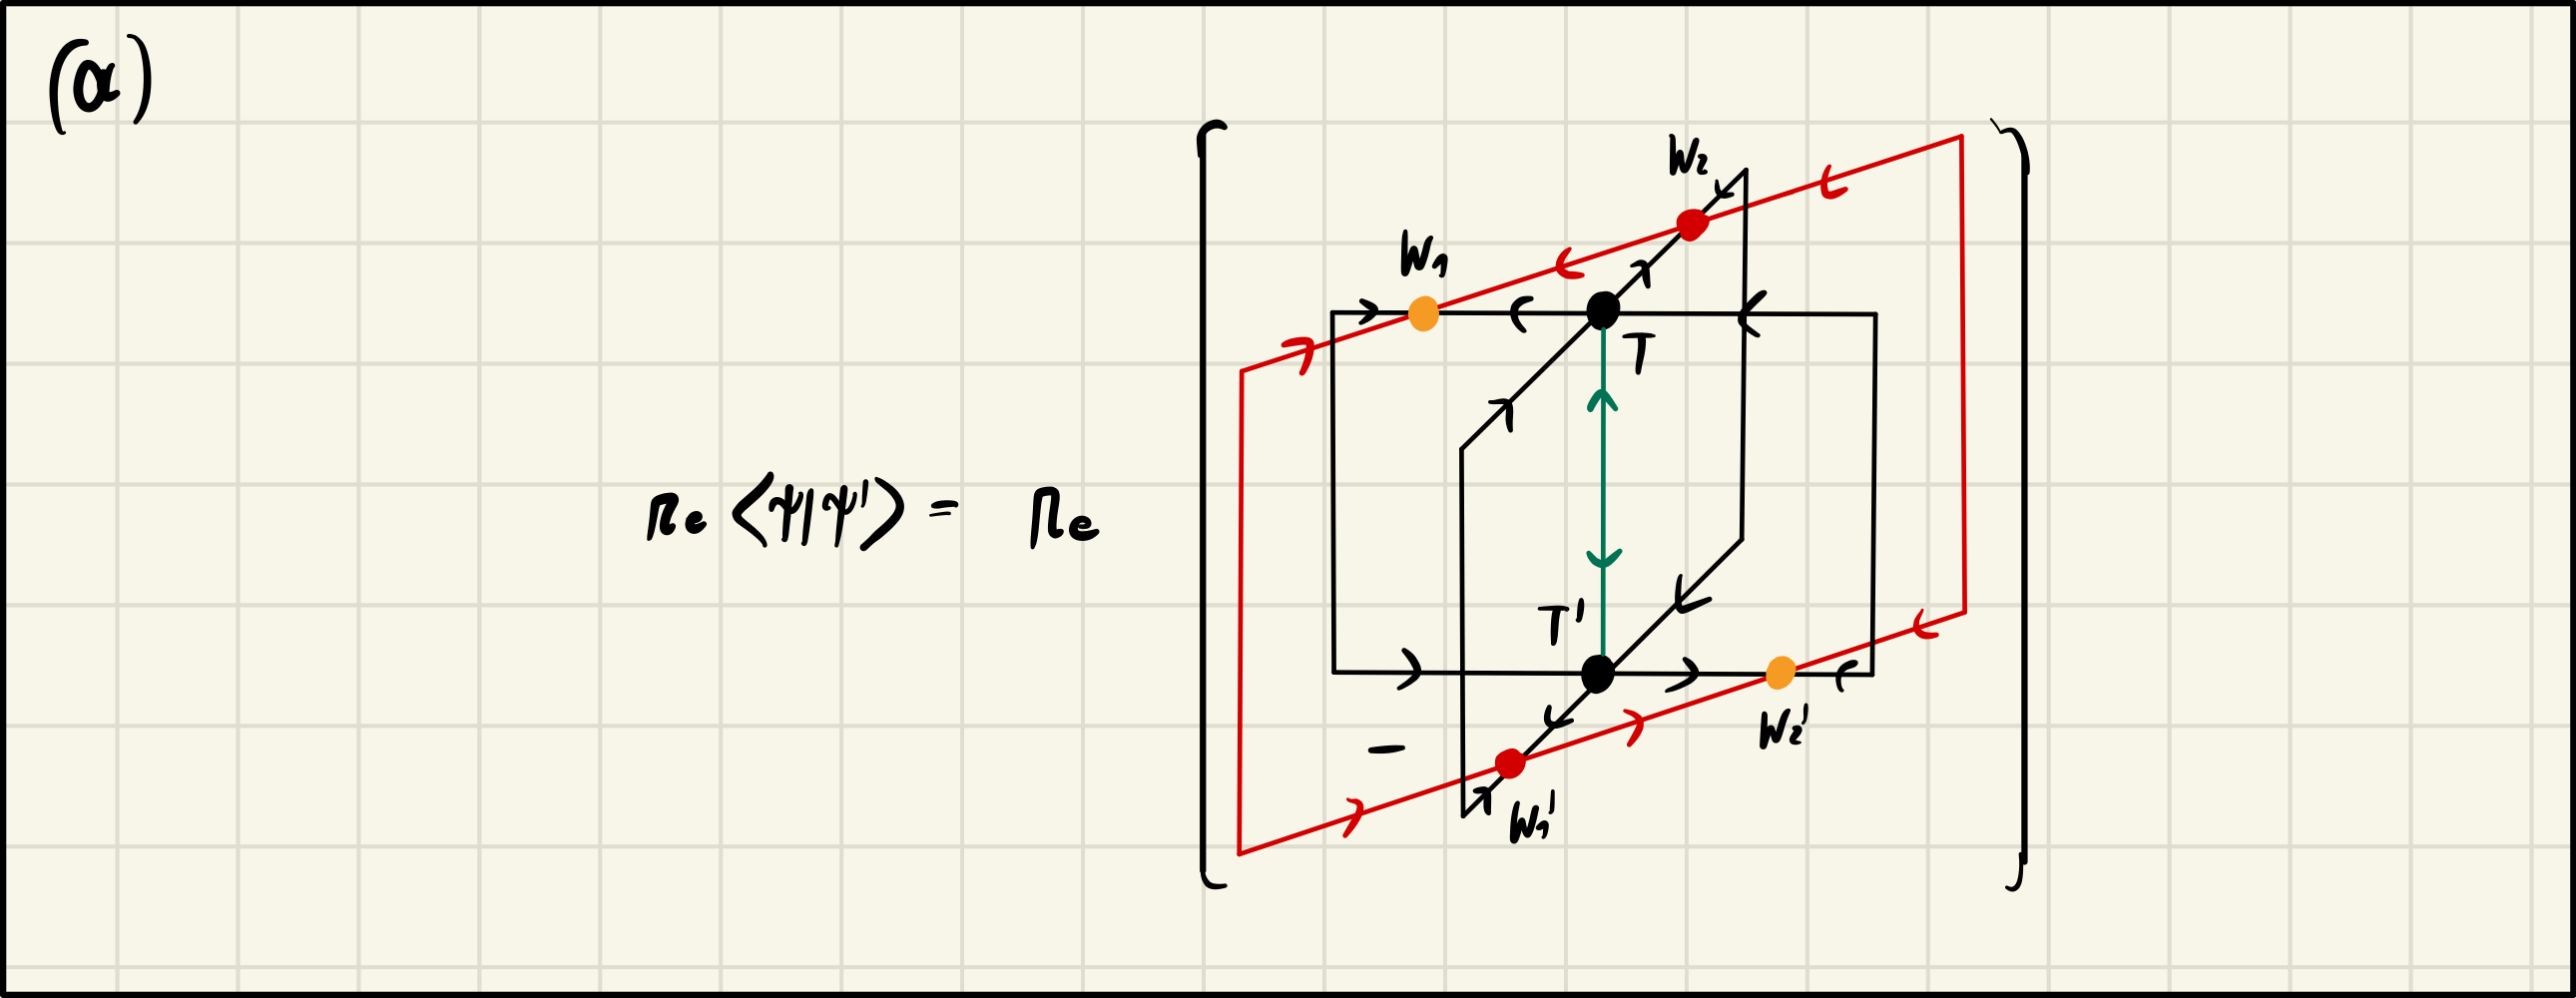
\includegraphics[width=0.6\textwidth]{figures/disoTPS/YB_move_iterate_polar_a.jpeg}
	}
	\subcaptionbox{\label{fig:YB_move_iterate_polar_optimize_W2}}
	{%
		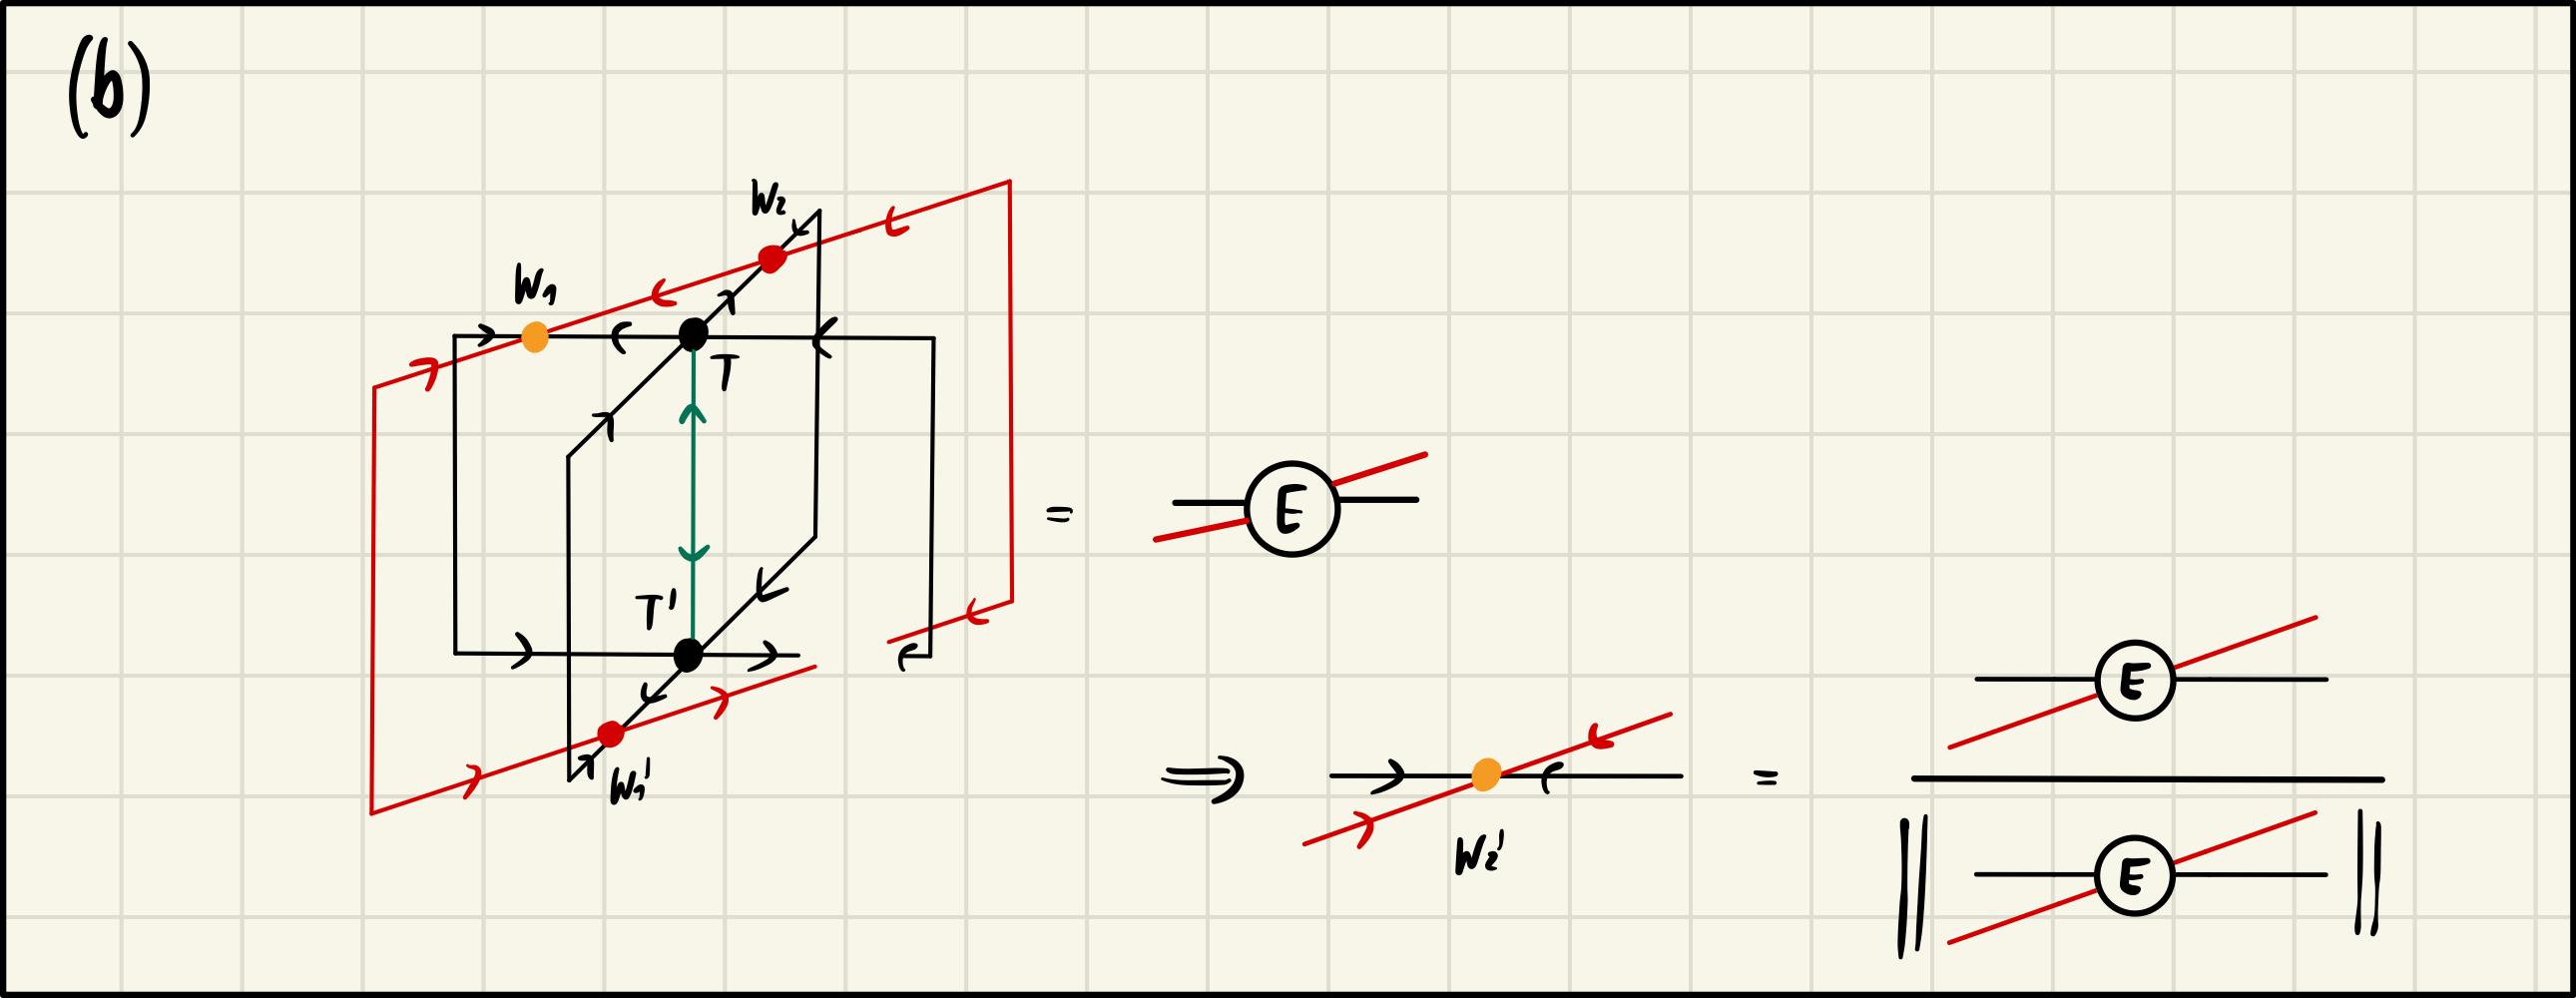
\includegraphics[width=0.6\textwidth]{figures/disoTPS/YB_move_iterate_polar_b.jpeg}
	}
	\subcaptionbox{\label{fig:YB_move_iterate_polar_optimize_W1}}
	{%
		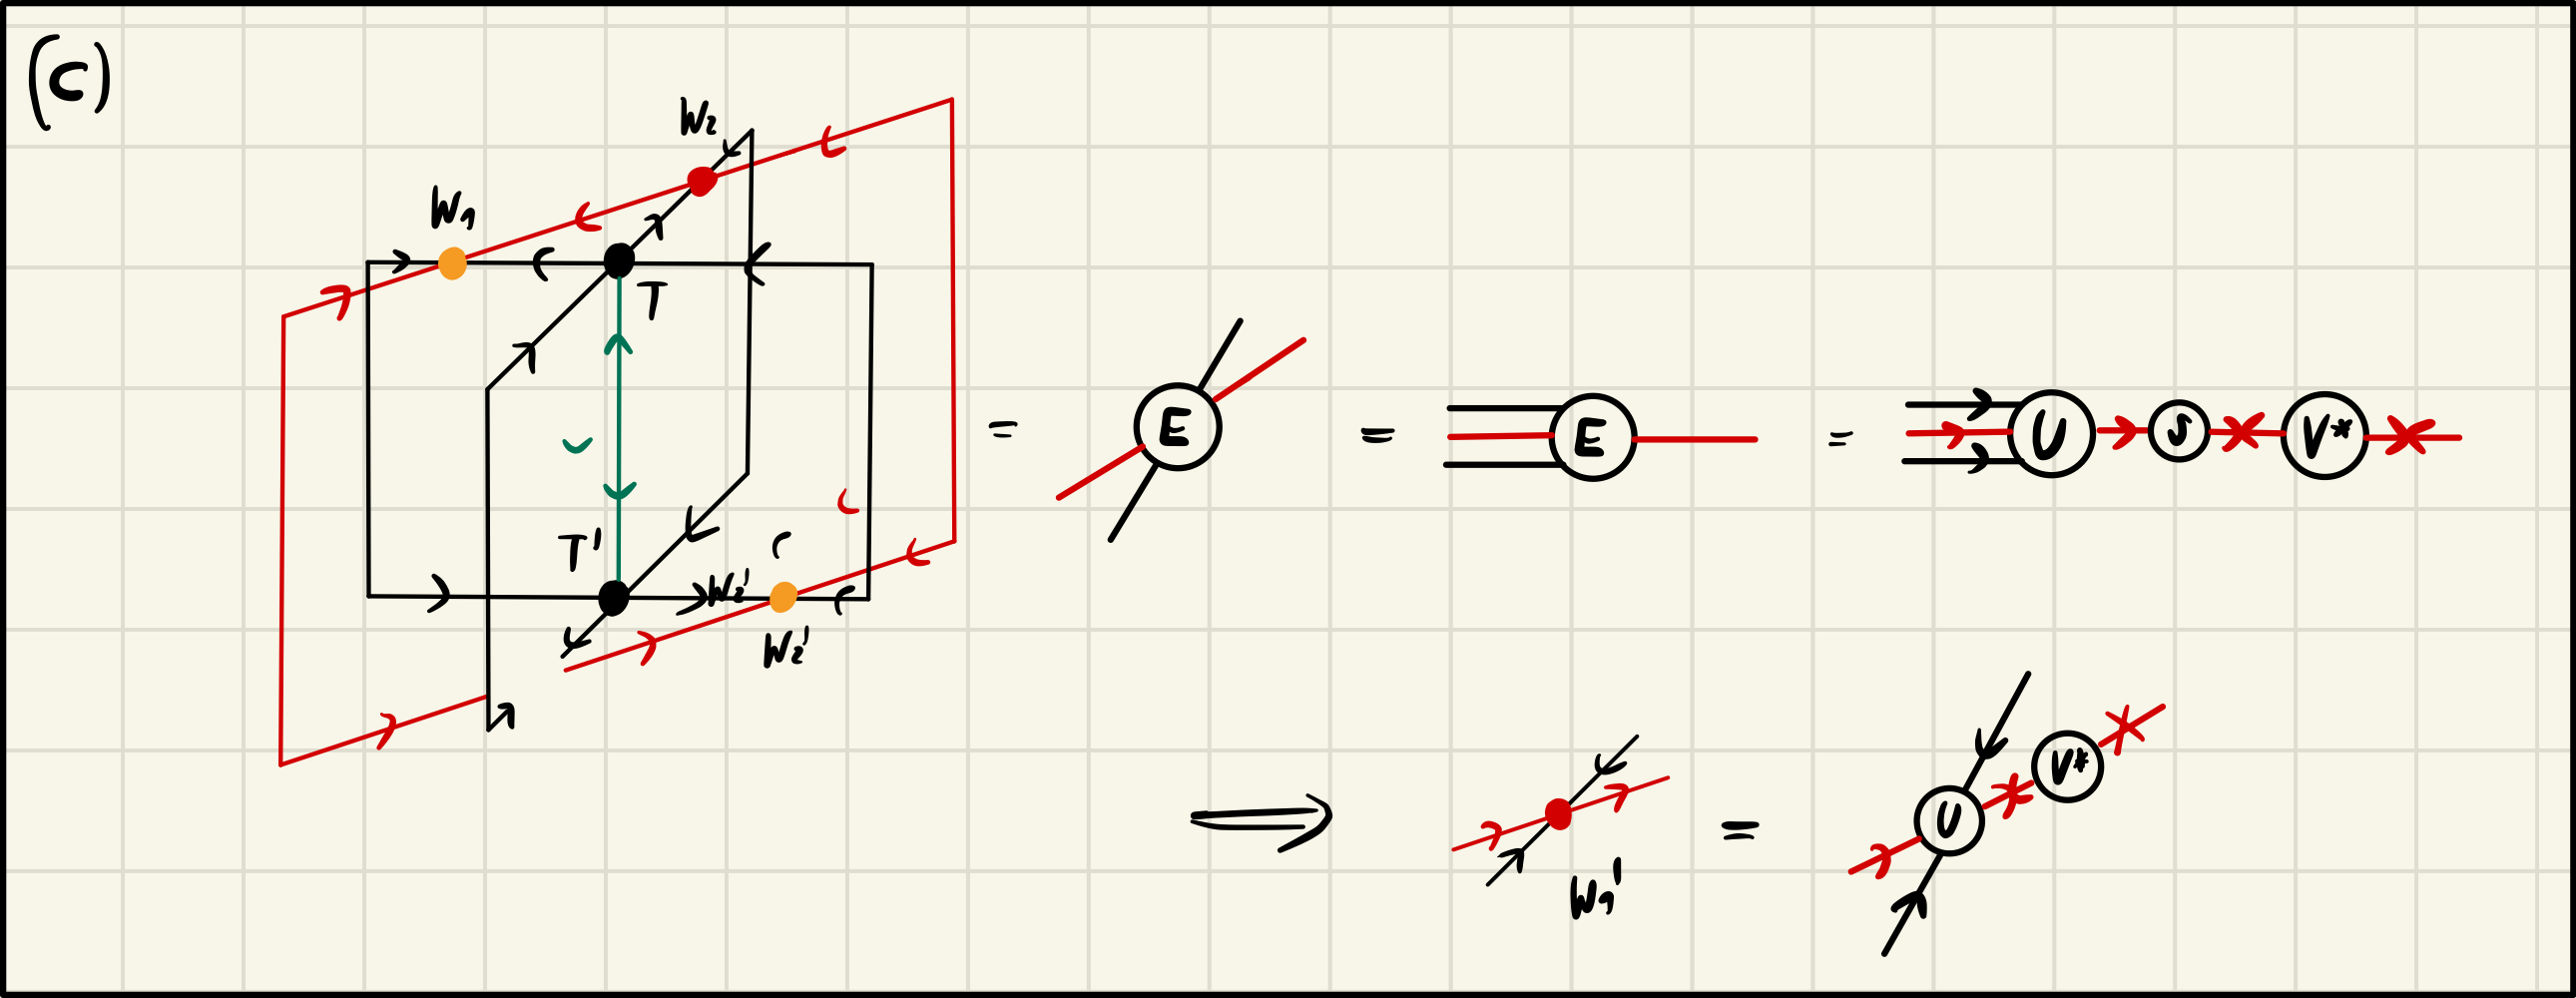
\includegraphics[width=0.6\textwidth]{figures/disoTPS/YB_move_iterate_polar_c.jpeg}
	}
	\subcaptionbox{\label{fig:YB_move_iterate_polar_optimize_T}}
	{%
		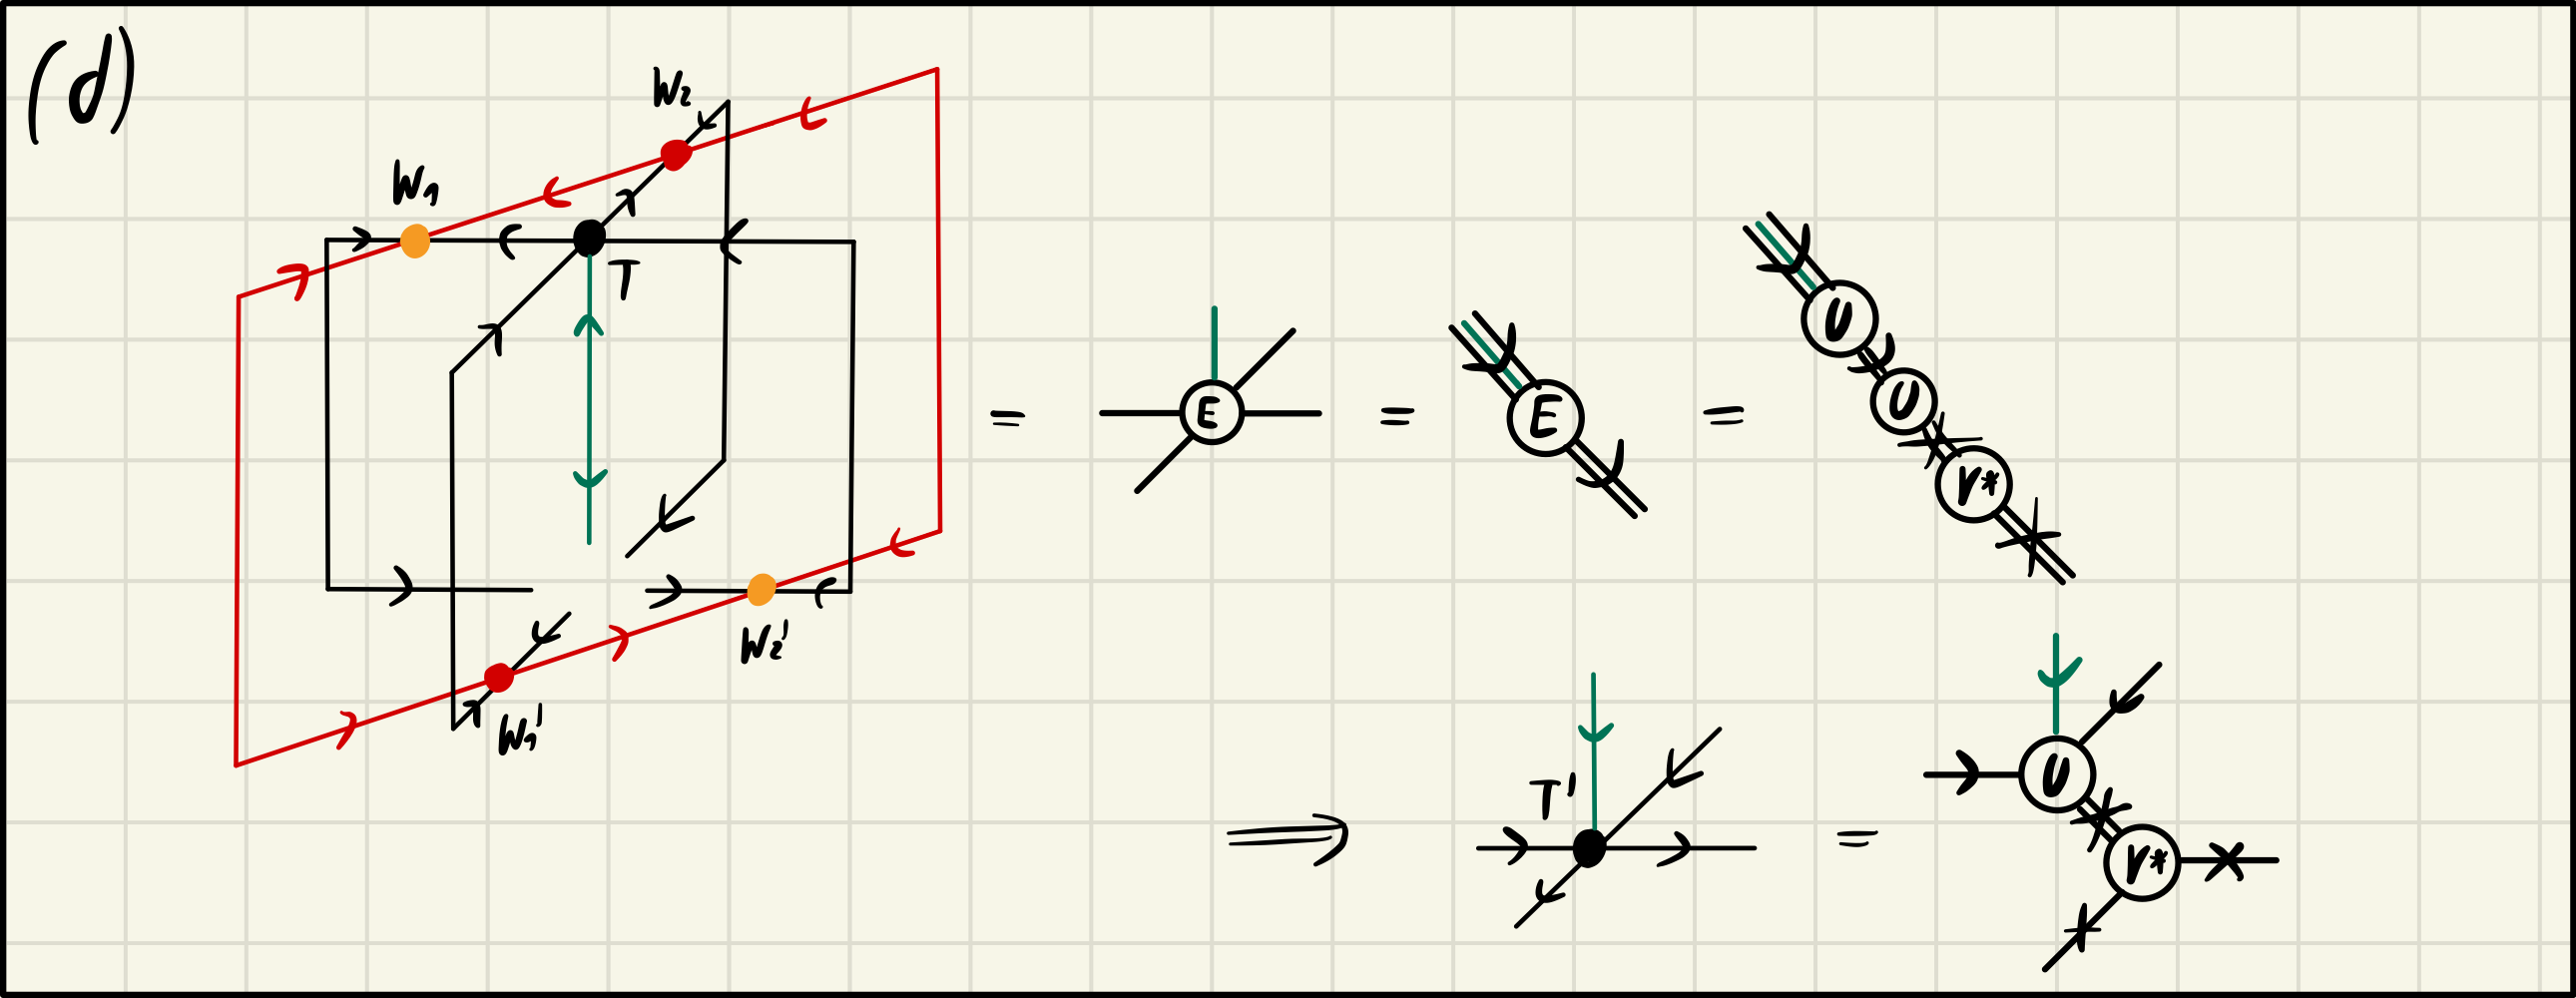
\includegraphics[width=0.6\textwidth]{figures/disoTPS/YB_move_iterate_polar_d.jpeg}
	}
	\caption{(a) The cost function of the optimization problem \eqref{eq:disoTPS_YB_move_alternative_formulation} can be computed as a contraction of only six tensors. (b) To optimize the tensor $W_2^\prime$, all tensors except $W_2^\prime$ are contracted into the environment $E$. The updated tensor is then given as $W_2^\prime = E/\lVert E\rVert$. (c) The tensor $W_1^\prime$ can be updated by contracting all tensors except $W_1^\prime$ into the environment $E$, which is subsequently isometrized using an SVD. (d) The tensor $T^\prime$ can be updated similarly by contracting all tensors except $T^\prime$ into the environment $E$ and isometrizing $E$ using an SVD.}
	\label{fig:YB_move_iterate_polar}
\end{figure}